% Ejemplo de documento LaTeX
% Tipo de documento y tamaño de letra
\documentclass[12pt]{article}


\usepackage[spanish]{babel}
\usepackage{longtable} 
\selectlanguage{spanish}
\usepackage[utf8x]{inputenc}
\usepackage{graphicx}




% EL titulo, autor y fecha del documento
\title{Reporte de Actividad 5}
\author{Carlos Medina}
\date{03-03-15}


% Aqui comienza el cuerpo del documento
\begin{document}
% Construye el título
\maketitle


El siguiente reporte describirá los pasos realizados para la actividad 5 (2015-1), se explicarán y se mostrarán los resultados de ésta.




\hspace {0.5cm} El $Tiro Parabolico$ es una forma de movimiento en el que un objeto o partícula (llamado proyectíl) es arrojado cerca de la superficie terrestre, y se mueve alrededor del trayecto de una curva bajo la acción de la gravedad sólamente. La única fuerza significante que actúa sobre el objeto es la gravedad, que actúa hacia abajo a causa de una aceleración hacia el centro de la Tierra. No hay fuerzas horizontales necesarias para mantener el movimiento horizontal – coherente con el concepto de inercia. 

El movimiento parabólico puede ser analizado como la composición de dos movimientos rectilíneos: un movimiento rectilíneo uniforme horizontal y un movimiento rectilíneo uniformemente acelerado vertical.
La trayectoria balística es la trayectoria de vuelo que sigue un proyectil sometido únicamente a su propia inercia y a las fuerzas inherentes al medio en el que se desplaza, principalmente la fuerza gravitatoria. La ciencia que estudia los fenómenos balísticos en general se denomina balística. La balistica exterior estudia la trayectoria balística bajo diversas condiciones.

Si el proyectil fue lanzado con una velocidad inicial $Vo$, entonces se puede describir con la expresión:

\begin{center}
	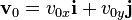
\includegraphics[width=3.5cm]{velin.png}\\
\end{center}

Los componentes $Vox$ y $Voy$ pueden ser encontrados si el angulo $0$ es conocido:

\begin{center}
	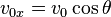
\includegraphics[width=3cm]{velx.png}\\
\end{center}
\begin{center}
	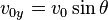
\includegraphics[width=3cm]{vely.png}\\
\end{center}

% Nunca debe faltar esta última linea.
\end{document}
